\newproblem{18.5a}
{
	Graph the quadratic function with the characteristics below.  Be sure to label the appropriate points on the graph.
	\begin{itemize}
	\item	Vertex: $(-4,1)$  
	\item $y$-intercept: $y=-3$ 
	\item $x$-intercepts: $x=-2,-6$
	\item Axis of symmetry: $x=-4$
	\end{itemize}
	\begin{onlyproblem}\begin{center}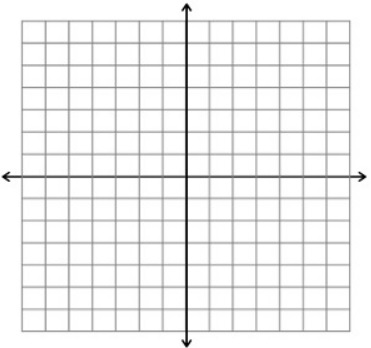
\includegraphics{fig-graphpaper.png}\end{center}\end{onlyproblem} \begin{onlysolution}\begin{center}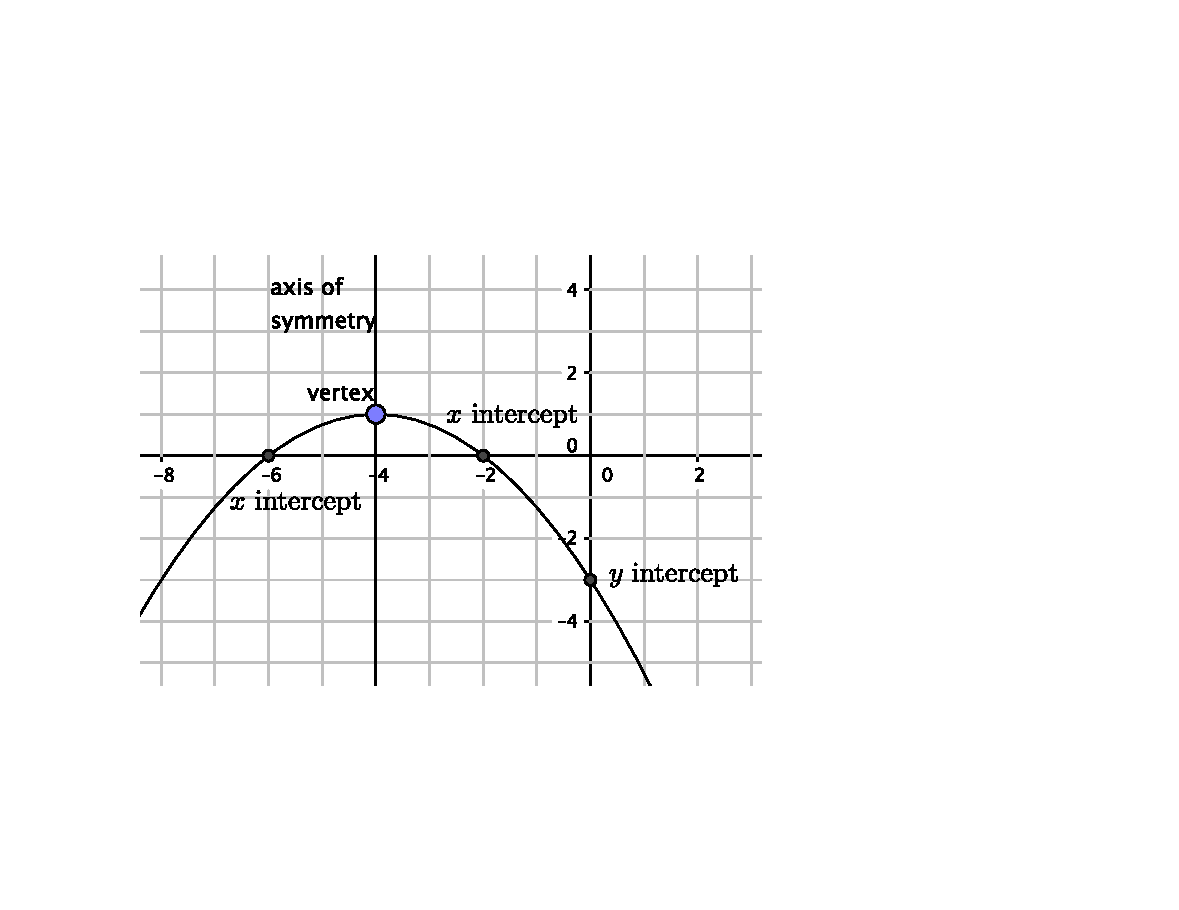
\includegraphics{fig100-18_5-a-answer}\end{center}\end{onlysolution}}
{
	\begin{tabular}{l r}
	Plot the vertex correct&1 point\\
	Plot the $x$-intercepts& Add 2 pts\\
	Plot the $y$-intercept & Add 1 pt\\
	Have a concave down parabola&Add 2 pts\\
	Label the points&Add 2 pts
	\end{tabular}
}

\newproblem{18.5b}
{
	Graph the quadratic function with the characteristics below.  Be sure to label the appropriate points on the graph.
	\begin{itemize} 
	\item	Vertex: $(2,5)$  
	\item $y$-intercept: $y=4.2$ 
	\item $x$-intercepts: $x=-3,7$
	\item Axis of symmetry: $x=2$
	\end{itemize}
	\begin{onlyproblem}\begin{center}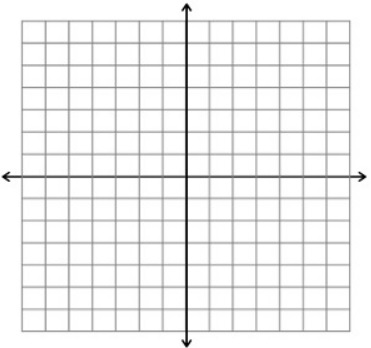
\includegraphics{fig-graphpaper.png}\end{center}\end{onlyproblem} \begin{onlysolution}\begin{center}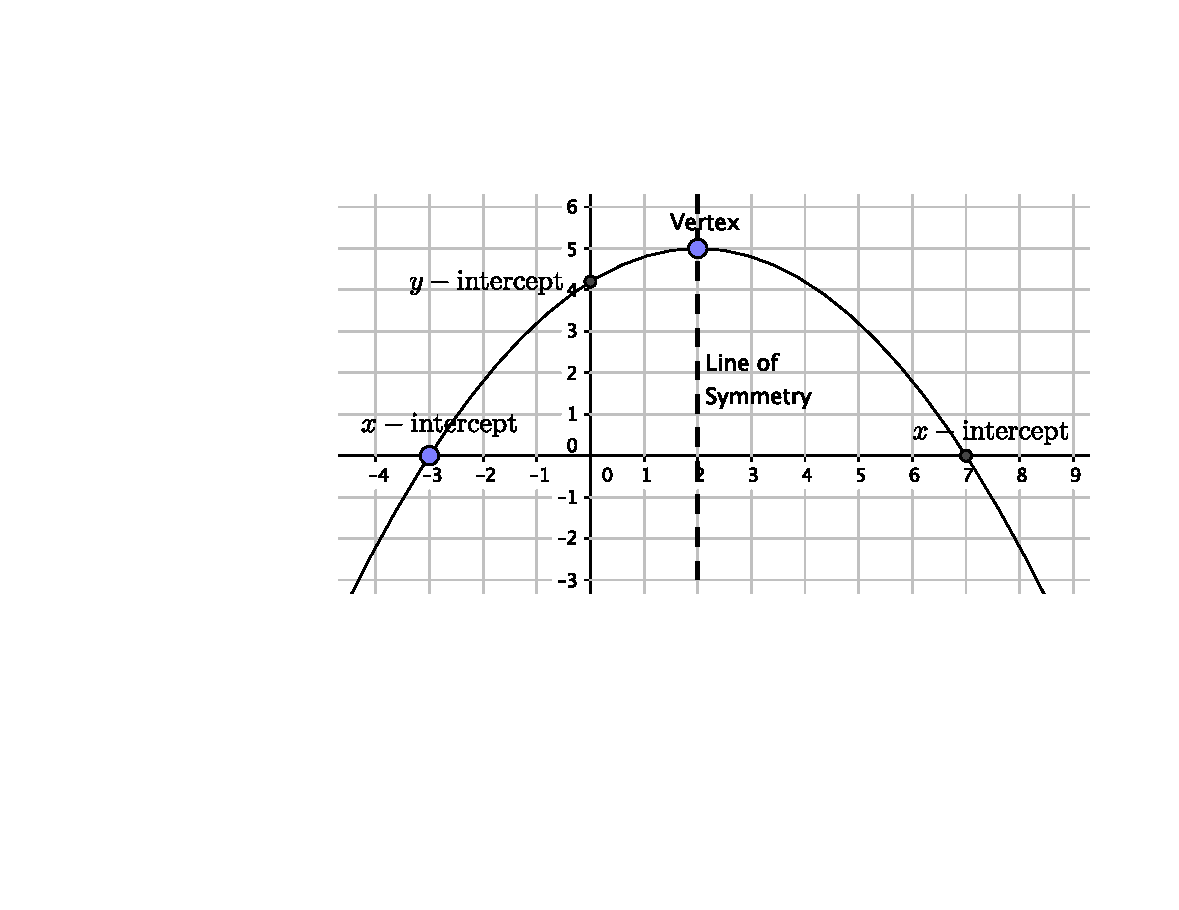
\includegraphics{fig100-18_5-b-answer}\end{center}\end{onlysolution}}
{
	\begin{tabular}{l r}
	Plot the vertex correct&1 point\\
	Plot the $x$-intercepts& Add 2 pts\\
	Plot the $y$-intercept & Add 1 pt\\
	Have a concave down parabola&Add 2 pts\\
	Label the points&Add 2 pts
	\end{tabular}
}

\newproblem{18.5c}
{
	Graph the quadratic function with the characteristics below.  Be sure to label the appropriate points on the graph.
	\begin{itemize}
	\item	Vertex: $(-5,-1)$  
	\item $y$-intercept: $y=5.25$ 
	\item $x$-intercepts: $x=-3,-75$
	\item Axis of symmetry: $x=-5$
	\end{itemize}
	\begin{onlyproblem}\begin{center}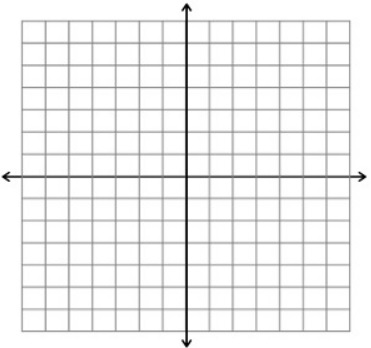
\includegraphics{fig-graphpaper.png}\end{center}\end{onlyproblem} \begin{onlysolution}\begin{center}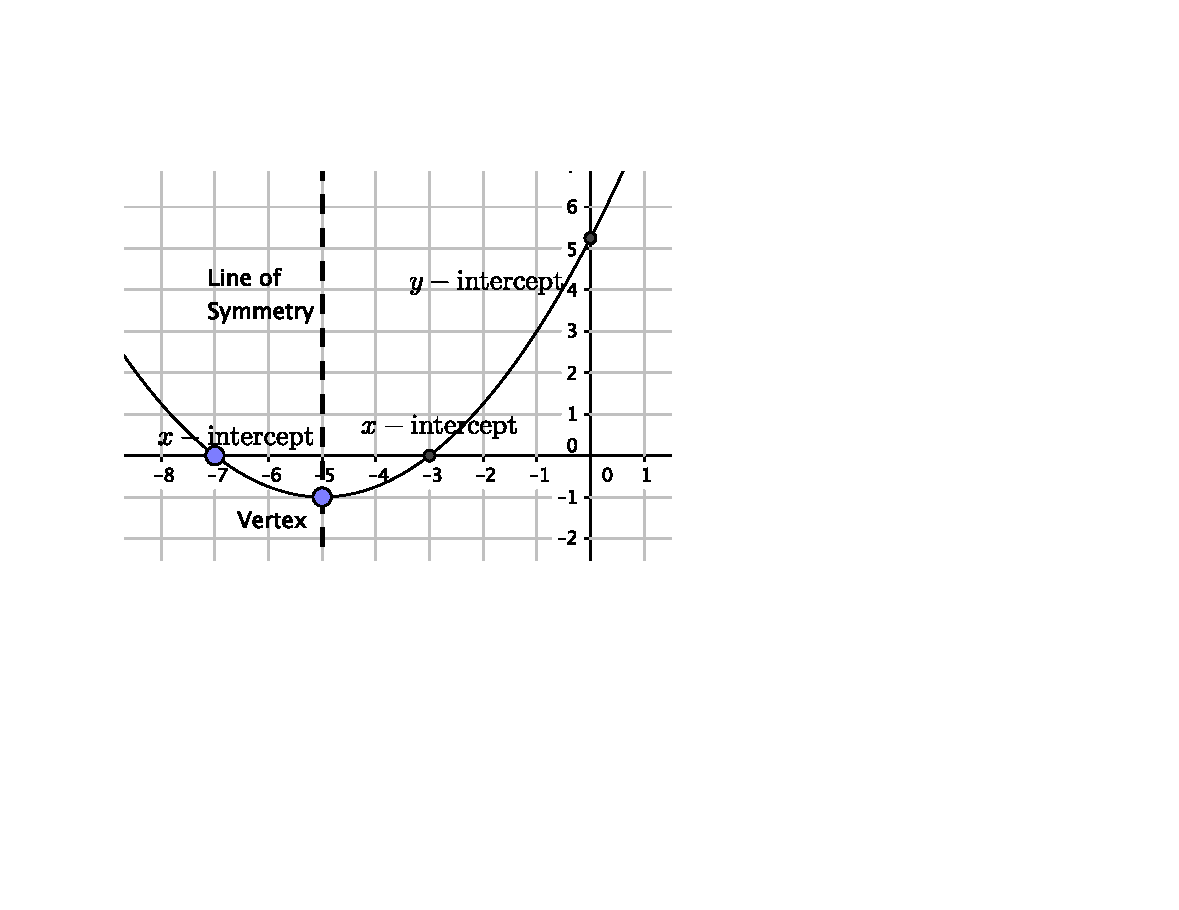
\includegraphics{fig100-18_5-c-answer}\end{center}\end{onlysolution}}
{
	\begin{tabular}{l r}
	Plot the vertex correct&1 point\\
	Plot the $x$-intercepts& Add 2 pts\\
	Plot the $y$-intercept & Add 1 pt\\
	Have a concave down parabola&Add 2 pts\\
	Label the points&Add 2 pts
	\end{tabular}
}
\newproblem{18.5d}
{
	Graph the quadratic function with the characteristics below.  Be sure to label the appropriate points on the graph.
	\begin{itemize}
	\item	Vertex: $(2,-8)$  $y=.5(x+2)(x-6)$
	\item $y$-intercept: $y=-6$ 
	\item $x$-intercepts: $x=-2,6$
	\item Axis of symmetry: $x=2$
	\end{itemize}
	\begin{onlyproblem}\begin{center}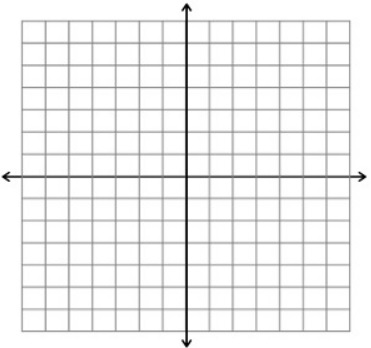
\includegraphics{fig-graphpaper.png}\end{center}\end{onlyproblem} \begin{onlysolution}\begin{center}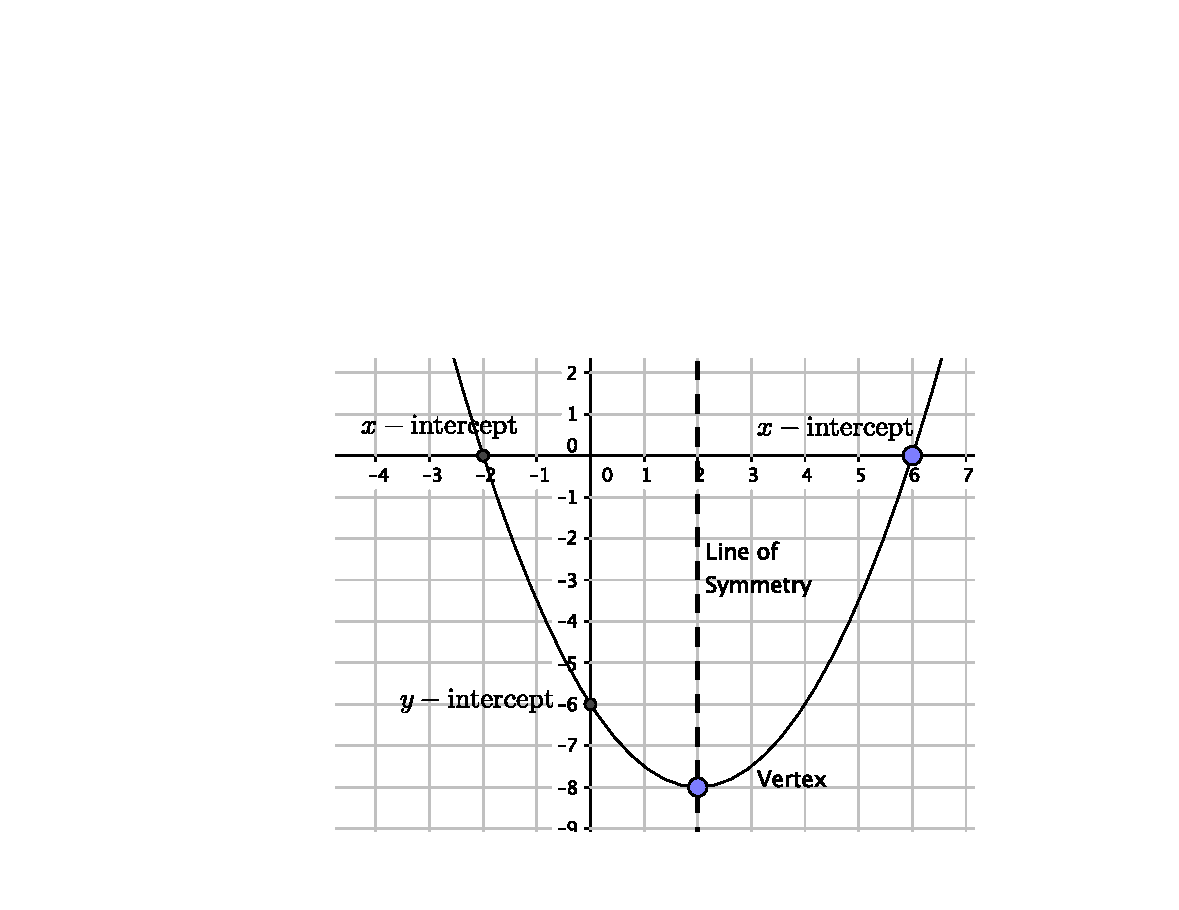
\includegraphics{fig100-18_5-d-answer}\end{center}\end{onlysolution}}
{
	\begin{tabular}{l r}
	Plot the vertex correct&1 point\\
	Plot the $x$-intercepts& Add 2 pts\\
	Plot the $y$-intercept & Add 1 pt\\
	Have a concave down parabola&Add 2 pts\\
	Label the points&Add 2 pts
	\end{tabular}
}